% ------------------------------------------------------------------------
% file `3_uaa2_2023-2024-appliquer-5-exercise-body.tex'
%   in folder `xsim/'
%
%     exercise of type `appliquer' with id `5'
%
% generated by the `appliquer' environment of the
%   `xsim' package v0.21 (2022/02/12)
% from source `3_uaa2_2023-2024' on 2023/12/06 on line 61
% ------------------------------------------------------------------------
    Détermine les longueurs demandées (elles sont notées par le symbole "?"). Note bien tout ton raisonnement de façon structurée et rigoureuse.
    \begin{tasks}
        \task 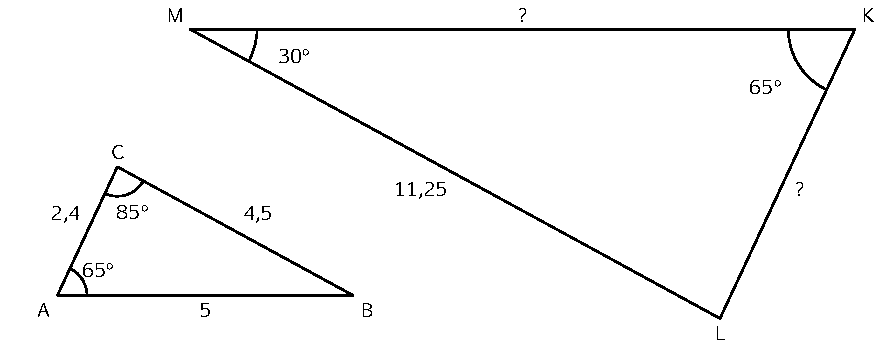
\includegraphics[valign=t]{tikz/sim_01.pdf}%3
        \task 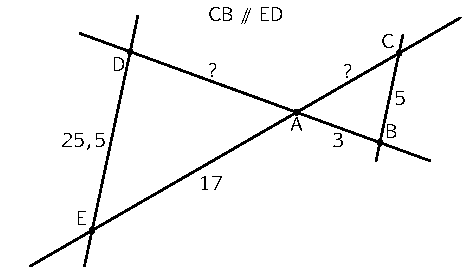
\includegraphics[valign=t]{tikz/thales_01.pdf}%2
        \task 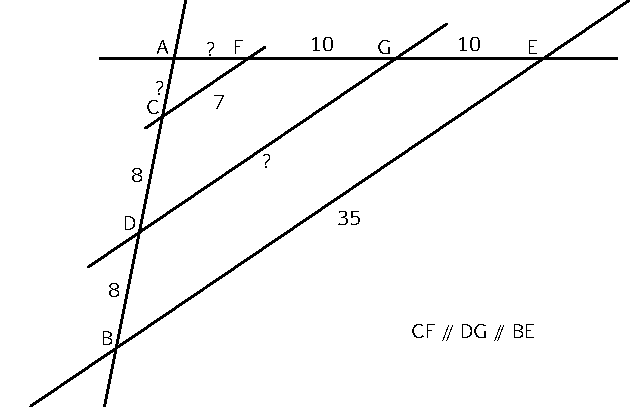
\includegraphics[valign=t]{tikz/thales_02.pdf}%3
        \task 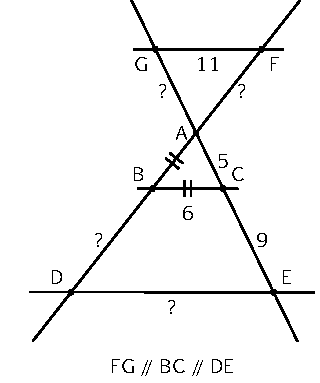
\includegraphics[valign=t]{tikz/thales_03.pdf}%4
    \end{tasks}
